\documentclass[b5paper,xelatex,ja=standard,10pt]{bxjsarticle}
\usepackage{mystyle}  % export TEXINPUTS="./;../sty/;"
\graphicspath{{../images/}}

\usepackage{listings}
\lstset{  % グローバル設定
  columns=fixed,  % 等幅
  basewidth=0.5em,  % 字間詰め
  lineskip=-3pt,  % 行間詰め
  % フォント設定
  basicstyle={\ttfamily\small\color{DarkGray}},  % 全体設定
  keywordstyle=[1]{\color{RoyalBlue}},  % kewords[1]の設定 (Python だと予約語)
  keywordstyle=[2]{\color{VioletRed}},  % kewords[2]の設定 (Python だと組み込み関数)
  stringstyle={\color{FireBrick}},  % 文字列リテラルの設定
  commentstyle={\color{SeaGreen}},  % コメントの設定
}

\makeatletter
\renewcommand*\l@section{\@dottedtocline{1}{0.0em}{4.0em}}
\makeatother

\usepackage{eso-pic}

\newcommand\BackgroundPic{%
\put(0,0){%
\parbox[b][\paperheight]{\paperwidth}{%
\vfill
\centering
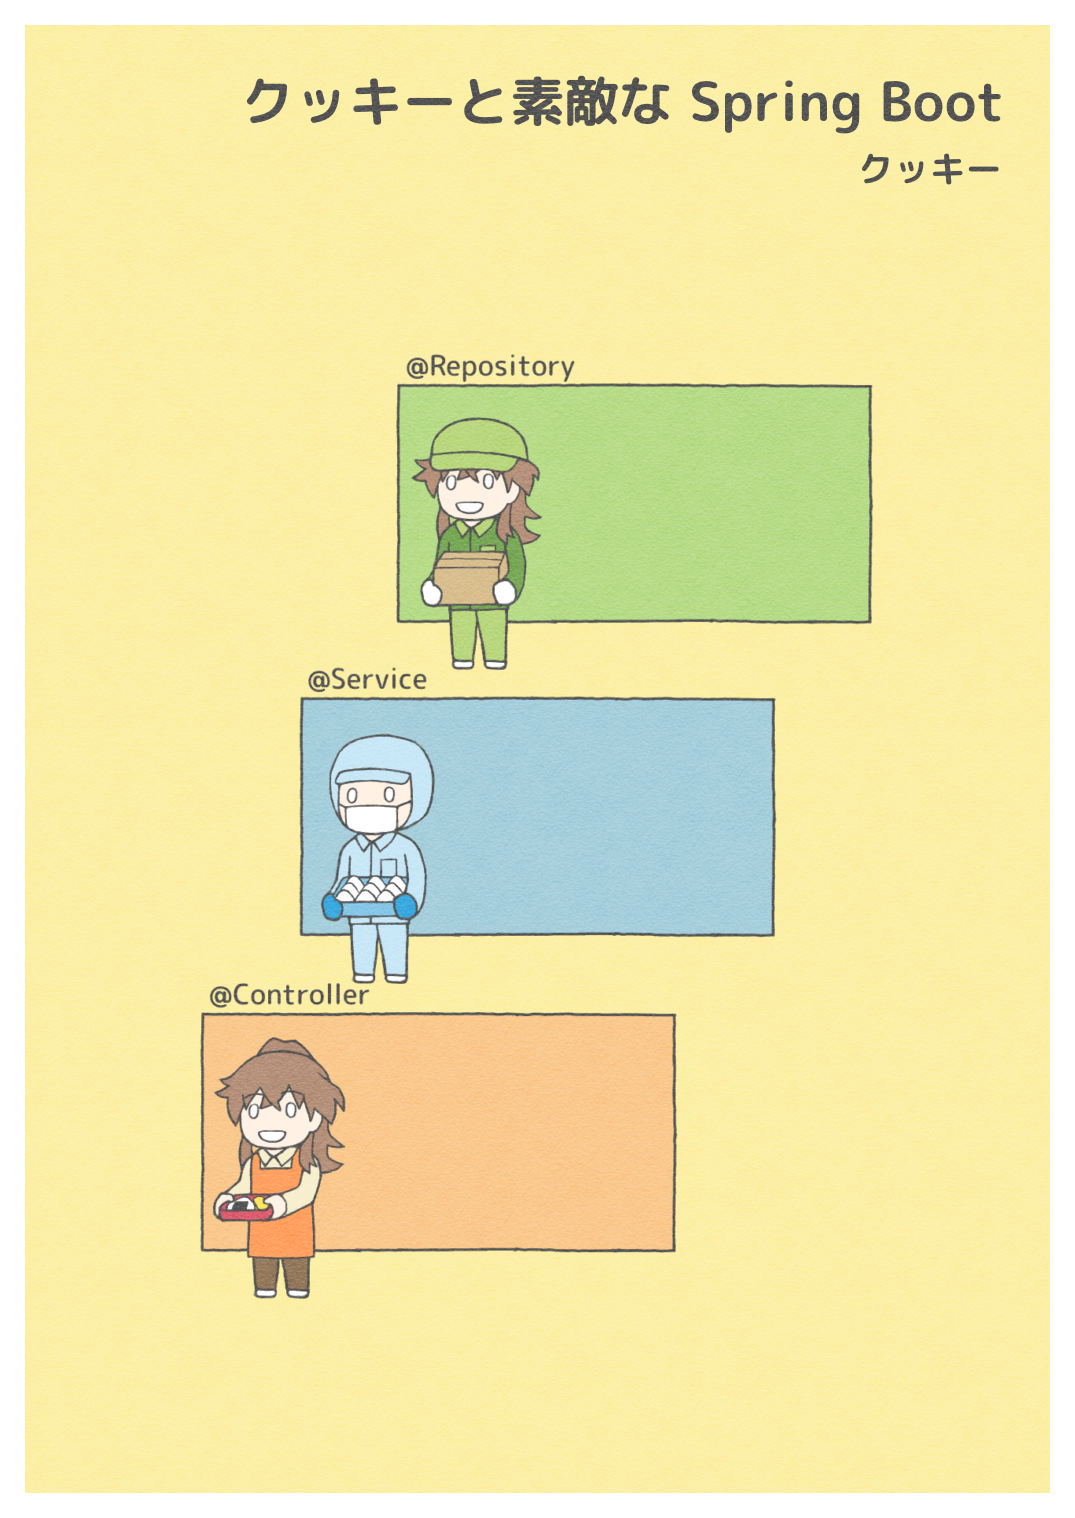
\includegraphics[width=1.0\paperwidth,height=1.0\paperheight,%
keepaspectratio]{cover.png}%
\vfill
}}}

\newcommand*{\mywatermark}{\addfontfeatures{Color=Teal} \textbf{\small DRAFT 2022-01-30 \\ \url{https://github.com/CookieBox26/notes/tree/main/20211226_spring_boot} }}
\renewcommand*{\mywatermark}{}
\AddToShipoutPictureBG{
  \AtPageUpperLeft{
    \raisebox{-2.2\baselineskip}{\makebox[\paperwidth]{\begin{minipage}{14cm}\centering{\mywatermark}\end{minipage}}}
  }
}



\begin{document}

% タイトル画像
\AddToShipoutPicture*{
  \BackgroundPic
  \AtPageLowerLeft{
    \raisebox{2.7\baselineskip}{\makebox[\paperwidth]{\begin{minipage}{14cm}\centering{\mywatermark}\end{minipage}}}
  }
  \AtPageUpperLeft{
    \raisebox{-5.7\baselineskip}{\makebox[\paperwidth]{\begin{minipage}{15.4cm}\leftline{{\addCJKfontfeatures{Color=MediumVioletRed} \textbf{\huge \, \, \, \,   未完成ドラフト}}}\end{minipage}}}
  }
  \AtPageUpperLeft{
    \raisebox{-8.8\baselineskip}{\makebox[\paperwidth]{
    \begin{minipage}{0.9\paperwidth}{
        \addfontfeatures{Color=MediumVioletRed}
        \addCJKfontfeatures{Color=MediumVioletRed}
        {\large
        \hspace{7.6em}この本は未完成ドラフトです。 \\
        \hspace{7.6em}目次の内容をかくことを目指しましたが \\
        \hspace{7.6em}全然完成しませんでした。
        }
    }\end{minipage}
  }}
  }
}
\begin{titlepage}
\ 
\end{titlepage}


% 地の文の文字色をグレーに変更する
\addfontfeatures{Color=DarkGray}
\addCJKfontfeatures{Color=DarkGray}


% 目次
\begin{spacing}{1.1}
\textbf{\tableofcontents}
\end{spacing}


\section*{まえがき}
\addcontentsline{toc}{section}{まえがき}
\vspace{3pt}

以下の JDK を使用しています。
\begin{itemize}
\item openjdk 11.0.13 2021-10-19
\item OpenJDK Runtime Environment Temurin-11.0.13+8 (build 11.0.13+8)
\item OpenJDK 64-Bit Server VM Temurin-11.0.13+8 (build 11.0.13+8, mixed mode)
\end{itemize}

以下のパッケージを使用しています。
\begin{itemize}
\item Spring Boot 2.6.1
\end{itemize}

本書の内容についてお気付きの点がありましたら、大変お手数ですが、この本のコードか原稿のリポジトリの Issues、または著者ブログのコメント欄までお知らせください。著者ブログへのコメントはただちには公開されません。非公開希望の方はその旨をお知らせください。非公開希望であって返信が必要な場合はご連絡先の明記をお願いいたします。

\begin{description}
   \item[ コードリポジトリ] https://github.com/CookieBox26/bentou-application
   \item[ 原稿リポジトリ] https://github.com/CookieBox26/notes/
   \begin{itemize}
       \item この本のディレクトリは 20211226\_spring\_boot です。
   \end{itemize}
   \item[ 著者ブログ] https://cookie-box.hatenablog.com/
\end{description}

\vspace{6pt}
%\subsubsection*{登場人物紹介}
\centerline{\textbf{登場人物(の代理)紹介}}

\vspace{3pt}
\begin{SERIFU}[colback=White, colbacktitle=PaleIris2, top=-1pt, bottom=0pt, left=18pt, right=10pt]{kazusa_smiley.png}
\small
この人はベイズ統計部の部長ですが、この本ではクッキーの代理として登場します。この人がベイズ統計部の部長として出てくるお話は他の本を参照してください。
\end{SERIFU}

\newcounter{mycounter}
\stepcounter{mycounter}
\newcommand*{\mysectiontitle}{クッキー、Spring Boot 開発に参加する}
\section*{第{\themycounter}話 \, \mysectiontitle}
\addcontentsline{toc}{section}{\numberline {第{\themycounter}話}\mysectiontitle}
\vspace{3pt}

\begin{SERIFU}[colback=PaleIris, colbacktitle=PaleIris2]{kazusa_worried.png}
Spring Boot (Java)による REST API 開発に参加することになりました。Python でならいくつかのやり方で REST API を実装したことがありますが、Spring Boot は触ったことがありません。そもそも Java での開発も初めてに等しいです。Java モジュールに数行の修正 PR をしたことは何度かありますが、機能追加をするなどは経験がないので、Java における開発プラクティスの知見もまるでありません。
\end{SERIFU}

\begin{SERIFU}[colback=PaleIris, colbacktitle=PaleIris2]{kazusa_neutral.png}
……まあしかし、REST API であるならばコードをみれば何が何なのかは概ねわかるでしょう。今回の私のタスクは何もスクラッチで REST API を構築することではありません。{\addCJKfontfeatures{Color=VioletRed}{\addfontfeatures{Color=VioletRed}現在既に「弁当」を返却しているベントウAPIがあり、リクエストに応じてその「弁当」に「卵焼き」を追加する}}だけです。外部 API から新たに「卵」を取り寄せる必要はありますが――。
\end{SERIFU}

\begin{SERIFU}[colback=PaleIris, colbacktitle=PaleIris2]{kazusa_smile.png}
ともかく適当なソースファイルをみてみましょう――どのファイルも1行目に
\begin{CODE}[title=\texttt{src/main/java/com/example/bentou/BentouApplication.java}]
\begin{lstlisting}[language=java]
package com.example.bentou;
\end{lstlisting}
\end{CODE}
などとありますね。これは「このソースファイル内に定義されているクラスは com.example.bentou なるパッケージに所属しています」という意味ですか。クラスを適宜パッケージに整理せよということですね。
\end{SERIFU}

\begin{SERIFU}[colback=PaleIris, colbacktitle=PaleIris2]{kazusa_smile.png}
では、HTTP リクエストを受け取るハンドラはどこにあるのでしょうか?  現在の仕様書によると {\addfontfeatures{Color=FireBrick}/bentou} なるエンドポイントに HTTP GET することで「弁当」が返却されるはずですが……あっ、このクラスでしょうか。
\begin{CODE}[title=\texttt{src/main/java/com/example/bentou/BentouController.java}]
\begin{lstlisting}[language=java,emph={@RestController,@Autowired,@Qualifier,@GetMapping},emphstyle=\color{VioletRed}]
package com.example.bentou;

import org.springframework.beans.factory.annotation.Autowired;
import org.springframework.beans.factory.annotation.Qualifier;
import org.springframework.web.bind.annotation.GetMapping;
import org.springframework.web.bind.annotation.RestController;

@RestController
public class BentouController {
    private final OnigiriService onigiriService;

    @Autowired
    public BentouController(
        @Qualifier("tuna") OnigiriService onigiriService
    ) {
        this.onigiriService = onigiriService;
    }

    @GetMapping("/bentou")
    public Bentou provide() {
        Bentou bentou = new Bentou();
        bentou.onigiri = this.onigiriService.provideOnigiri();
        return bentou;
    }
}
\end{lstlisting}
\end{CODE}
{\addfontfeatures{Color=VioletRed}@GetMapping}({\addfontfeatures{Color=FireBrick}"/bentou"}) が付加されたメソッド(Python でいうデコレータのようですが――?)がリクエストを受け取っておにぎりを返却しているようにみえます。このメソッドがリクエストハンドラとみていいでしょう。
\end{SERIFU}


\stepcounter{mycounter}
\renewcommand*{\mysectiontitle}{クッキー、最大の謎に直面する}
\section*{第{\themycounter}話 \, \mysectiontitle}
\addcontentsline{toc}{section}{\numberline {第{\themycounter}話}\mysectiontitle}


\begin{SERIFU}[colback=PaleIris, colbacktitle=PaleIris2]{kazusa_smile.png}
リクエストハンドラがわかればリクエストに応じて返却フィールドを追加する変更は実装できそうです。
\end{SERIFU}

\begin{SERIFU}[colback=PaleIris, colbacktitle=PaleIris2]{kazusa_worried.png}
……しかし、リクエストハンドラをもつ BentouController クラスがどこでインスタンス化されているのかさっぱりわかりません。リポジトリを grep してもそれらしき箇所がありません。BentouController クラスにはコンストラクタもあるようですし、やはりこれはインスタンス化して利用するものでしょう。であれば、何がどうなって――
\end{SERIFU}

\begin{SERIFU}[colback=PaleIris, colbacktitle=PaleIris2]{kazusa_neutral.png}
調べてみたところ、Spring Boot プロジェクトをビルドして実行すると、@SpringBootApplication 付きのクラスに対して、以下の 1. 2. のオブジェクトが勝手に生成されるのですね\cite{doc_annotation}。
\begin{enumerate}
  \item そのクラス自身 or そのパッケージ以下で @Configuration 付きで定義されたクラスがもつ @Bean 付きのメソッドが返すオブジェクト。
  \item そのパッケージ以下で @RestController, @Controller, @Service, @Repository, @Component 付きで定義されたクラスのインスタンス。 
  \begin{itemize}
      \item そもそも Spring には @Component しかなく、Spring Boot ではそのクラスの役割がリクエスト窓口 / ロジック / データ操作かに応じて @Controller / @Service / @Repository を使い分けるがクラスの役割の明確化以上の意味はないらしい \cite{review} \cite{kihon}。
  \end{itemize}
\end{enumerate}
1. 2. から生成されたオブジェクトを {\addfontfeatures{Color=VioletRed}Bean} とよぶのですね。自作クラスを Bean とするときは 2. の方法、サードパーティのクラスを Bean とするときは 1. の方法をとることになるようです \cite{chigai}。
\end{SERIFU}

\stepcounter{mycounter}
\renewcommand*{\mysectiontitle}{クッキー、Controller の単体テストで行き詰まる}
\section*{第{\themycounter}話 \, \mysectiontitle}
\addcontentsline{toc}{section}{\numberline {第{\themycounter}話}\mysectiontitle}

\begin{SERIFU}[colback=PaleIris, colbacktitle=PaleIris2]{kazusa_neutral.png}
MockMvc を用いるとリクエストに対するレスポンスが期待通りかのテストを実装できそうです \cite{test_mockmvc}。
\end{SERIFU}

\begin{SERIFU}[colback=PaleIris, colbacktitle=PaleIris2]{kazusa_neutral.png}
しかし、このとき Bean を本番用のものと置き換えたいですね \cite{bean}。
\end{SERIFU}


\stepcounter{mycounter}
\renewcommand*{\mysectiontitle}{クッキー、RestTemplate の利用に行き詰まる}
\section*{第{\themycounter}話 \, \mysectiontitle}
\addcontentsline{toc}{section}{\numberline {第{\themycounter}話}\mysectiontitle}

\begin{SERIFU}[colback=PaleIris, colbacktitle=PaleIris2]{kazusa_neutral.png}
外部APIのレスポンス形式が JSON のとき、XML のときにレスポンスをパースするにはどうすればいいのでしょうか。
\end{SERIFU}


\stepcounter{mycounter}
\renewcommand*{\mysectiontitle}{クッキー、Service の単体テストで行き詰まる}
\section*{第{\themycounter}話 \, \mysectiontitle}
\addcontentsline{toc}{section}{\numberline {第{\themycounter}話}\mysectiontitle}

\begin{SERIFU}[colback=PaleIris, colbacktitle=PaleIris2]{kazusa_neutral.png}
外部APIをモックするには MockRestServiceServer が使えそうです。
\end{SERIFU}


\stepcounter{mycounter}
\renewcommand*{\mysectiontitle}{クッキー、サーキットブレーカーに嫌われる}
\section*{第{\themycounter}話 \, \mysectiontitle}
\addcontentsline{toc}{section}{\numberline {第{\themycounter}話}\mysectiontitle}

\begin{SERIFU}[colback=PaleIris, colbacktitle=PaleIris2]{kazusa_neutral.png}
サーキットブレーカーとは、外部へのアクセスが失敗し続けている状況のときに遮断できる仕組みなのですね \cite{cb}。交通整理員さんのようなものでしょうか? 遮断している状態は電気回路でいうと途切れてしまっている状態 (解放) ですから、「オープン」なのですね。
\end{SERIFU}


\stepcounter{mycounter}
\renewcommand*{\mysectiontitle}{クッキー、接続プールが不足する}
\section*{第{\themycounter}話 \, \mysectiontitle}
\addcontentsline{toc}{section}{\numberline {第{\themycounter}話}\mysectiontitle}

\begin{SERIFU}[colback=PaleIris, colbacktitle=PaleIris2]{kazusa_neutral.png}
要求仕様通りに実装できたと思いきや、リクエスト数を捌いてくれませんね。いったいなぜ――
\end{SERIFU}

\begin{SERIFU}[colback=PaleIris, colbacktitle=PaleIris2]{kazusa_neutral.png}
org.apache.http.impl.conn.PoolingHttpClientConnectionManager が接続プール数をつかさどっているのですね。予め上限をゆるめた PoolingHttpClientConnectionManager を用意する必要がありそうです。
\end{SERIFU}


\stepcounter{mycounter}
\renewcommand*{\mysectiontitle}{クッキー、メトリクスを隠される}
\section*{第{\themycounter}話 \, \mysectiontitle}
\addcontentsline{toc}{section}{\numberline {第{\themycounter}話}\mysectiontitle}


\stepcounter{mycounter}
\renewcommand*{\mysectiontitle}{クッキーと素敵な Spring Boot}
\section*{第{\themycounter}話 \, \mysectiontitle}
\addcontentsline{toc}{section}{\numberline {第{\themycounter}話}\mysectiontitle}

\begin{SERIFU}[colback=PaleIris, colbacktitle=PaleIris2]{kazusa_neutral.png}
Spring Boot プロジェクトの開発とは、必要な Bean たちを用意し、適宜 Bean に他の Bean を持たせることだと思いました。
\end{SERIFU}

\begin{SERIFU}[colback=PaleIris, colbacktitle=PaleIris2]{kazusa_neutral.png}
Spring Boot プロジェクトを会社に、各 Bean を部署に喩えるなら以下です。
\end{SERIFU}

\includegraphics[keepaspectratio, scale=0.56]{bentou.png}


\addcontentsline{toc}{section}{参考文献}
\begin{thebibliography}{99}
    \bibitem{review} Spring Bootアプリケーションのコードレビューポイント - Qiita, \url{https://qiita.com/cross-xross/items/144f8bde2ef6fa4b379f}, 参照日:2022年1月30日.
    \bibitem{kihon} 【Spring】@Autowired と @Component を使用した DI の基本 - 山崎屋の技術メモ, \url{https://www.shookuro.com/entry/2016/08/09/175801}, 参照日:2022年1月30日.
    \bibitem{doc_annotation} Spring Boot での開発 - リファレンスドキュメント \#6. @SpringBootApplication アノテーションの使用, \url{https://spring.pleiades.io/spring-boot/docs/current/reference/html/using.html#using.using-the-springbootapplication-annotation}, 参照日:2022年1月30日.
    \bibitem{chigai} Spring Bootの@Componentと@Beanの違い - grep Tips *, \url{https://www.greptips.com/posts/1318/}, 参照日:2022年1月30日.
    \bibitem{test_mockmvc} Spring Boot MockMvc と @MockBean で Web レイヤーテスト - 公式サンプルコード, \url{https://spring.pleiades.io/guides/gs/testing-web/}, 参照日:2022年1月30日.
    \bibitem{bean} 雑記: テスト時に Bean を別の Bean に置き換えたい話 - クッキーの日記, \url{https://cookie-box.hatenablog.com/entry/2021/12/05/124520}, 参照日:2022年1月30日.
    \bibitem{cb} 雑記: Circuit Breaker をオープンさせるだけ (resilience4j-spring-boot2) - クッキーの日記, \url{https://cookie-box.hatenablog.com/entry/2021/12/13/040728}, 参照日:2022年1月30日.
\end{thebibliography}


% 奥付
\clearpage
\vspace*{16.5cm} % 16.7
 \textbf{\large クッキーと素敵な Spring Boot}
\vspace*{-0.27cm}
\begin{OKUDUKE}[title={未完成ドラフト}]
2021年1月30日 初版発行 \\
%YYYY年MM月DD日 第2版発行 (まだ) \\
{
\renewcommand\arraystretch{0.9}
\begin{tabular}{p{4cm}rp{5.9cm}}
 &  &  \\
 & 著 者 & クッキー \\
 & 発行者 & クッキーの日記 \\
 & & https://cookie-box.hatenablog.com/ 
\end{tabular}
}
\end{OKUDUKE}
\thispagestyle{empty}


\end{document}
